\documentclass{article}
\usepackage{ctex}
\usepackage{amsmath,amscd,amsbsy,amssymb,latexsym,url,bm,amsthm}
\usepackage{epsfig,graphicx,subfigure}
\usepackage{enumitem,balance,mathtools}
\usepackage{wrapfig}
\usepackage{mathrsfs, euscript}
\usepackage[usenames]{xcolor}
\usepackage{hyperref}
\usepackage{caption}
\usepackage{setspace}
%\usepackage{subcaption}
\usepackage{float}
\usepackage{listings}
%\usepackage{enumerate}
%\usepackage{algorithm}
%\usepackage{algorithmic}
%\usepackage[vlined,ruled,commentsnumbered,linesnumbered]{algorithm2e}
\usepackage[ruled,lined,boxed,linesnumbered]{algorithm2e}
\usepackage{tikz}

\newtheorem{theorem}{Theorem}[section]
\newtheorem{lemma}[theorem]{Lemma}
\newtheorem{proposition}[theorem]{Proposition}
\newtheorem{corollary}[theorem]{Corollary}
\newtheorem{exercise}{Exercise}[section]
\newtheorem*{solution}{Solution}

\renewcommand{\thefootnote}{\fnsymbol{footnote}}
\renewenvironment{solution}[1][Solution]{~\\ \textbf{#1.}}{~\\}

\newcommand{\prob}{\mathtt{Pr}}

\newcommand{\postscript}[2]
{\setlength{\epsfxsize}{#2\hsize}
\centerline{\epsfbox{#1}}}

\newcommand{\dd}{\mathtt{d}}

\renewcommand{\baselinestretch}{1.0}
\SetKwFor{Function}{function}{:}{end}
\setlength{\oddsidemargin}{-0.365in}
\setlength{\evensidemargin}{-0.365in}
\setlength{\topmargin}{-0.3in}
\setlength{\headheight}{0in}
\setlength{\headsep}{0in}
\setlength{\textheight}{10.1in}
\setlength{\textwidth}{7in}

\title{计算方法\ 作业5}
\author{刘彦铭\ \ ID: 122033910081}
\date{Last Edited:\ \today}

\begin{document}

\maketitle

李庆杨等, 数值分析, 第5版, 华中科大, P.78,
13,14,16,17,20,22

\begin{spacing}{1.5}

\begin{itemize}
    \item [1.] 习题 13
    
    定义内积 $(f, g) = \int_0^{\pi/2} f(x)g(x) \dd x$, 设 $\psi_0=1, \psi_1=x$. $\left[\begin{array}{cc}(\psi_0, \psi_0)&(\psi_0, \psi_1)\\(\psi_1, \psi_0)&(\psi_1,\psi_1)\end{array}\right]\left[\begin{array}{c}b\\a\end{array}\right] = \left[\begin{array}{c}(f, \psi_0)\\(f, \psi_1)\end{array}\right]$,
    计算得到 $(\psi_0, \psi_0) = \pi/2$, $(\psi_0, \psi_1)=\pi^2/8$, $(\psi_1, \psi_1)=\pi^3/24$, $(f, \psi_0) = 1$, $(f, \psi_1) = 1$. 所以 
    
    
    $\left[\begin{array}{cc}\pi/2&\pi^2/8\\\pi^2/8&\pi^3/24\end{array}\right]\left[\begin{array}{c}b\\a\end{array}\right] = \left[\begin{array}{c}1\\1\end{array}\right]$
    解得: $a=\dfrac{96}{\pi^3}-\dfrac{24}{\pi^2}=0.664439$, $b = \dfrac{8}{\pi} - \dfrac{24}{\pi^2} = 0.114771$
    \item [2.] 习题 14
    
    \begin{itemize}
        \item [(1)] 不构成内积,因为 $(f, f) = \int_a^b f^\prime(x)g^\prime(x) \dd x = 0$ 不能推出 $f=0$.
        \item [(2)] 由微分积分的线性性可知 $(f, g) = \int_a^b f^\prime(x)g^\prime(x) \dd x + f(a)g(a)$ 的线性性显然,对称性也是显然的。
        关于正定性,显然 $(f, f) = \int_a^b f^\prime(x) f^\prime(x)\dd x + f(a)f(a) \geq 0$ 成立。而 由于 $\int_a^b f^\prime(x) f^\prime(x) \dd x \geq 0$,
        $f(a)f(a)\geq 0$, 所以 $(f, f) = 0$ 当且仅当 $\int_a^b f^\prime(x) f^\prime(x) \dd x = 0$ 且 $f(a)(a) = 0$, 这当且仅当 $f'(x) = 0, \forall x\in[a,b], f(a)=0 $, 当且仅当 在 [a, b] 上 有$f = 0$ .

        所以该定义构成内积。
    \end{itemize}

    \item [3.] 习题 16
    
    \begin{itemize}
        \item [(1)] $\int_{-1}^{1} (x - ax^2)^2 \dd x = \int_{-1}^1 x^2 -2ax^3 + a^2x^4 \dd x = \int_{-1}^1 x^2 \dd x + a^2\int_{-1}^1 x^4 \dd x$, $x^2, x^4$ 在 $[-1, 1]$ 上积分为正,故而 $a=0$ 时积分最小
        \item [(2)] 由于对称性,先只讨论 $a>0$ 的情形。
        
        当 $a > 1$ 即 $0 < 1/a < 1$ 时, $L=\int_{-1}^1 |x-ax^2|\dd x = \int_{-1}^0 (ax^2 - x)\dd x + \int_{0}^{\frac{1}{a}} (x - ax^2) \dd x + \int_{\frac{1}{a}}^{1} (ax^2 - x) \dd x = \dfrac{2}{3}a + \dfrac{1}{3a^2}$, $\dfrac{\dd L}{\dd a} = \dfrac{2}{a^3}(a^3-1)$, 当 $a>1$ 时递增,故其最小值在 $a\to 1$ 时取得。
        
        当 $0\leq a \leq 1$ 时, $L=\int_{-1}^1 |x-ax^2|\dd x = \int_{-1}^0 (ax^2 - x)\dd x + \int_{0}^{1} (x - ax^2) \dd x$, $\dfrac{\dd L}{\dd a} = \int_{-1}^0 x^2\dd x +\int_{0}^{1}-x^2 \dd x = 0$, 故当 $a\in[0, 1]$ 时积分取值都恒定。

        由上可知,取 $-1\leq a \leq 1$ 可使积分最小
    \end{itemize}

    \item [4.] 习题 17
    
    \begin{itemize}
        \item [(1)] 计算得到 $\left[\begin{array}{cc}(\varphi_1,\varphi_1)&(\varphi_1,\varphi_2)\\(\varphi_2,\varphi_1)&(\varphi_2,\varphi_2)\end{array}\right] = \left[\begin{array}{cc}1&1/2\\1/2&1/3\end{array}\right]$, $\left[\begin{array}{c}(\varphi_1, f)\\(\varphi_2, f)\end{array}\right]=\left[\begin{array}{c}1/3\\1/4\end{array}\right]$, 解得系数 $[a_1, a_2]^\top = [-\dfrac{1}{6}, 1]^\top$, 故而最佳平方逼近 $x - \dfrac{1}{6}$.
        \item [(2)] 计算得到  $\left[\begin{array}{cc}(\varphi_1,\varphi_1)&(\varphi_1,\varphi_2)\\(\varphi_2,\varphi_1)&(\varphi_2,\varphi_2)\end{array}\right] = \left[\begin{array}{cc}1/201&1/202\\1/202&1/203\end{array}\right]$, $\left[\begin{array}{c}(\varphi_1, f)\\(\varphi_2, f)\end{array}\right]=\left[\begin{array}{c}1/103\\1/104\end{array}\right]$, 解得系数 $[a_1, a_2]^\top = [ 375.2425, -375.1482]^\top$, 故而最佳平方逼近 $375.2425x^{100} -375.1482x^{101}$
        \item [比较:] (1) 中的逼近应该更好一些。一方面系数绝对值小,多项式次数低,计算方便,数值稳定;另一方面,(2) 中的逼近稍作变形即有 $375.2425x^{100} -375.1482x^{101} = 375.2425x^{100}(1-x) + \beta x^{101}$ 其中 $\beta$ 是一个约等于 $0.1$ 的系数,该函数的图像在接近 $1$ 时有一个非常陡峭的凸起, 而在$[0, 1]$ 上的大段区间内都接近于 $0$.
    \end{itemize}

    \item [5.] 习题 20
    
    \begin{itemize}
        \item [(1)] Legendre多项式逼近 $\left[\begin{array}{cccc}2&&&\\&2/3&&\\&&2/5&\\&&&2/7\end{array}\right]\left[\begin{array}{c}a_0\\a_1\\a_2\\a_3\end{array}\right] = \left[\begin{array}{c}0\\-4\cos (1/2)+8 \sin (1/2) \\ 0 \\ 236\cos (1/2) - 432 \sin (1/2)\end{array}\right]$ 解得 $[a_0, a_1, a_2, a_3]^\top = [0, -6\cos(1/2)+12\sin(1/2), 0, 826\cos(1/2) - 1512\sin(1/2)]^\top = [0, 0.487611, 0, -0.008218]^\top$, 
        
        故 $L(x) = 0.487611 x - 0.008218\left(\dfrac{5}{2}x^3 - \dfrac{3}{2}x\right)$, 图线如图\ref{Legendre}所示,这里用积分来计算均方误差,得到 $\delta = 9.75309\times 10^{-11}$
        
        \item [(2)] Chebyshev多项式逼近, $\rho(x)=\dfrac{1}{\sqrt{1-x^2}}$, $\left[\begin{array}{cccc}\pi&&&\\&\pi/2&&\\&&\pi/2&\\&&&\pi/2\end{array}\right]\left[\begin{array}{c}a_0\\a_1\\a_2\\a_3\end{array}\right] = \left[\begin{array}{c}0\\0.761109\\0\\-0.008054\end{array}\right]$, 解得 $[a_0,a_1,a_2,a_3]^\top = [0,0.484537,0,-0.005127]^\top$, 
        
        故 $T(x)=0.484537x-0.005127(4x^3-3x)$. 图线如图\ref{Chebyshev}所示,用积分计算均方误差,$\rho=1$ 对应于 $\delta=1.31349\times 10^{-10}$, $\rho=\dfrac{1}{\sqrt{1-x^2}}$对应于 $\delta=2.03939\times 10^{-10}$.
        
        \begin{figure}[htb]
            \begin{minipage}[t]{0.48\textwidth}
                \centering
                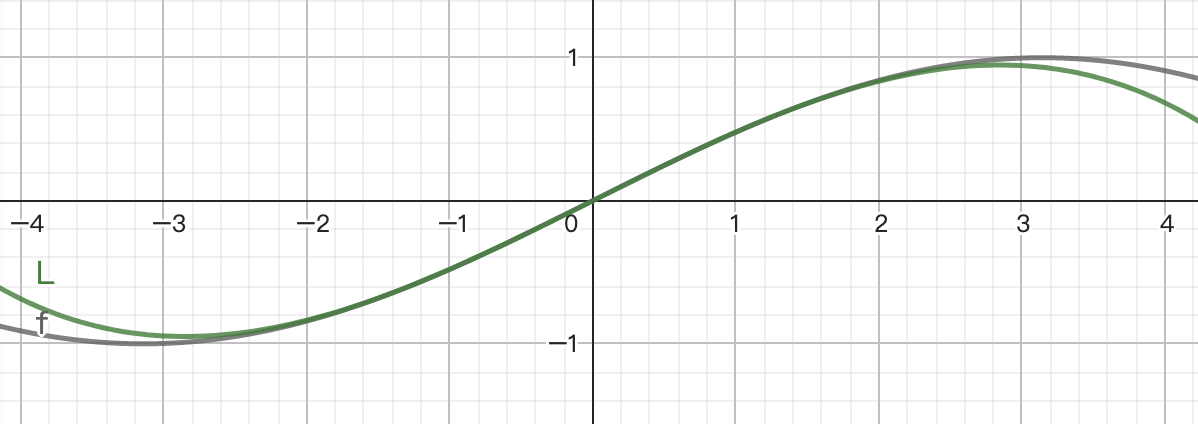
\includegraphics[width=0.96\textwidth]{截屏2022-12-03 16.16.31.png}
                \caption{Legendre 三次最佳平方逼近, 灰色是原函数, 绿色是三次逼近}
                \label{Legendre}
            \end{minipage}
            \begin{minipage}[t]{0.48\textwidth}
                \centering
                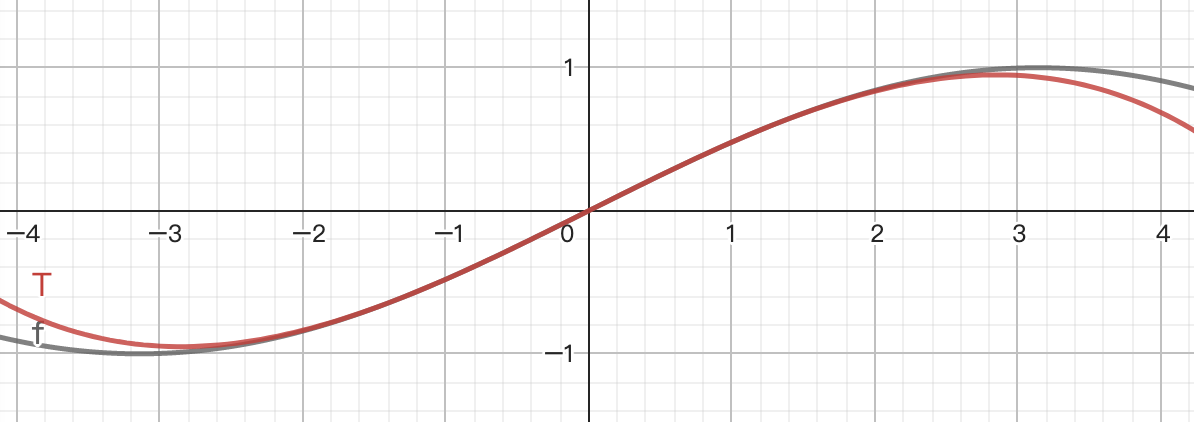
\includegraphics[width=0.96\textwidth]{截屏2022-12-03 16.44.00.png}
                \caption{Chebyshev 三次最佳平方逼近,灰色是原函数, 红色是三次逼近}
                \label{Chebyshev}
            \end{minipage}
        \end{figure}

        \begin{figure}[htb]
            \centering
            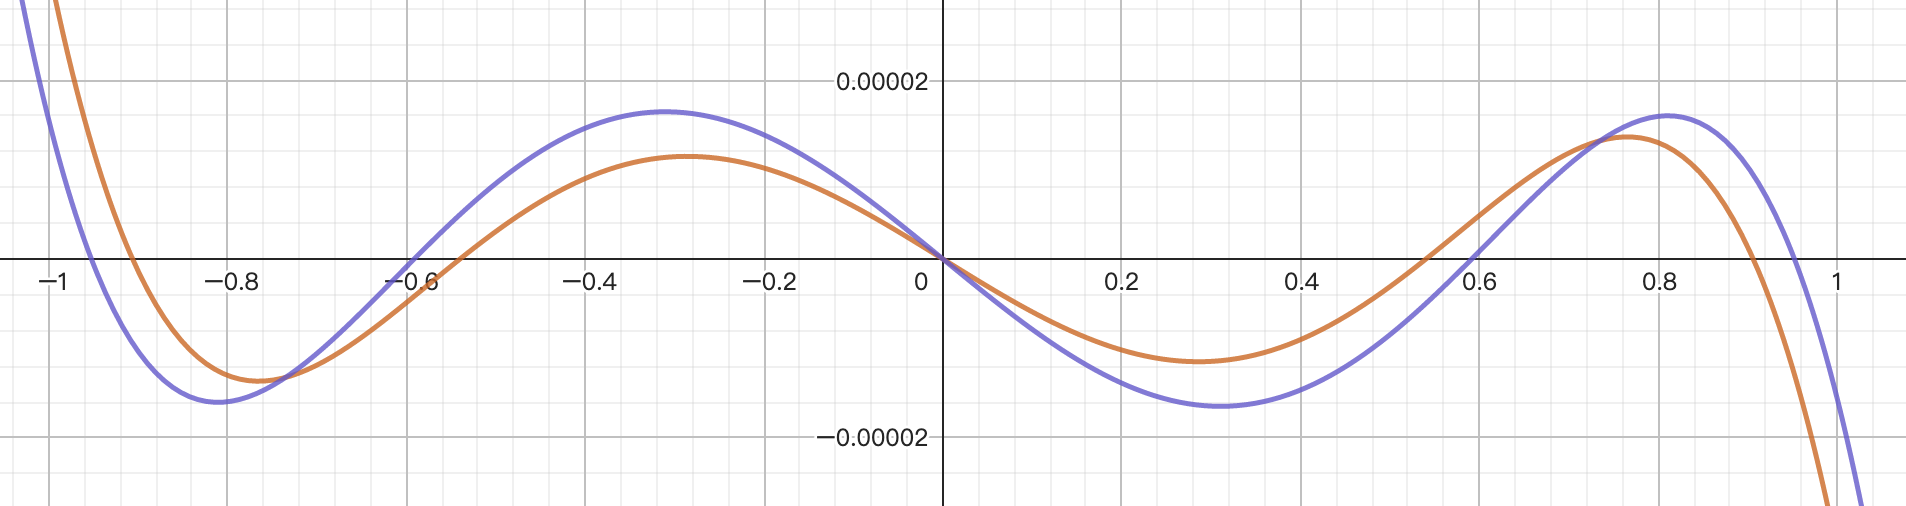
\includegraphics[width=0.85\textwidth]{截屏2022-12-03 17.13.31.png}
            \caption{误差图线。其中橙色的对应 Legendre多项式逼近, 紫色的对应 Chebyshev多项式逼近}
        \end{figure}
    \end{itemize}

    \item [6.] 习题 22
    
    只需将内积定义为离散形式 $(f, g) = \sum_{i} f(x_i)g(x_i)$. 计算得到 $\left[\begin{array}{cc}5 & 5327\\5327&7277699\end{array}\right]\left[\begin{array}{c}a\\b\end{array}\right] = \left[\begin{array}{c}271.4\\369321.5\end{array}\right]$, 得到 $[a, b]^\top = [0.97257866, 0.05003512]^\top$, $a + bx^2$. 数据点的函数值 $y=[19.0 , 32.3, 49.0 , 73.3, 97.8]^\top$, 拟合的对应点函数值 $\hat{y}=[19.03525698, 32.24452866, 49.05632898, 73.22329194, 97.84057098]^\top$, 计算得到 $||y-\hat{y}||_2 = 0.122569$, 均方误差 $\delta = \dfrac{1}{n}||y-\hat{y}||_2=0.0245138$

\end{itemize}
    
\end{spacing}

\end{document}